% Adapted by M-L. Messai
\documentclass[25pt, a0paper, portrait, margin=0mm, innermargin=15mm,blockverticalspace=15mm, colspace=15mm, subcolspace=8mm]{tikzposter}

\usepackage{pgfplots}


\usepackage[utf8]{inputenc}
\renewcommand{\refname}{Références}
\usepackage{lipsum} 
\usepackage{fancyhdr}
\usepackage[scaled]{helvet}
\renewcommand\familydefault{\sfdefault} 
\usepackage[T1]{fontenc}
\usepackage{transparent} % transparence des images

\usepackage{soulutf8} % surligner du texte
%\sethlcolor{} % couleur du surlignage

\usepackage[backend=biber,
    style=numeric-comp,
    maxcitenames=1,
    maxbibnames=1,
    %backref=true
    ]{biblatex}

\usepackage{colortbl} % colorer ligne d'un tableau
\usepackage{xspace}

\usepackage{tikz}
\usetikzlibrary{arrows,shapes}

\usepackage{enumitem} % changer les points de itemize


\tikzposterlatexaffectionproofoff %enlever phrase en bas à droite
\usetheme{Simple} %différents thèmes tikzposter

% ---- Couleurs
\definecolor{mypink1}{rgb}{0.858, 0.188, 0.478}
\definecolor{titlecolor}{RGB}{74, 114, 159}
\definecolor{titledarkcolor}{RGB}{51,102,153}
\definecolor{LightGrey}{RGB}{232, 232, 232}
\definecolor{Grey}{RGB}{222, 223, 225}
\definecolor{DarkerGrey}{RGB}{215,217,219}
\definecolor{FontColor}{RGB}{131,136,138}
\definecolor{Red}{RGB}{204,0,0}
%\definecolor{L-lig}{RGB}{25,124,192}
%\definecolor{eric-lab}{RGB}{54,104,163}
\definecolor{eric-lab}{RGB}{255,73,1} 
\definecolor{eric}{RGB}{255,255,255}



\definecolor{Orange}{RGB}{240,163,10} %ERIC orange
\definecolor{Gray}{RGB}{186,200,211}
\definecolor{LightRed}{RGB}{214,98,93}
\definecolor{LightBlue}{RGB}{160,200,217}
\definecolor{LightGreen}{RGB}{130,161,119}
\definecolor{Violet}{RGB}{190,144,252}
% ----

\colorlet{blocktitlefgcolor}{eric-lab} %titre des blocks
\colorlet{blocktitlebgcolor}{Grey} %couleur des lignes blocks
%\colorlet{blockbodybgcolor}{mypink1}%????
\colorlet{blockbodyfgcolor}{FontColor} %couleur du texte dans blocks

\colorlet{innerblocktitlefgcolor}{white}
\colorlet{notefrcolor}{Red!60} % ligne autour cadre notes
\colorlet{notefgcolor}{white} % couleur police notes
\colorlet{notebgcolor}{Red!60} % BG couleur des notes


% ---- Titre
\settitle{ 
\begin{minipage}[b]{0.8\linewidth}
\vspace{2cm}
\hspace{1cm}\color{black}{ \Huge\textsc{\textbf{\@title}} \par } \vspace*{2em} \hspace{1cm}\color{black}{\LARGE \@author \par} \vspace*{2em} \hspace{1cm}{\Large \@institute}\vspace{0.5cm} \end{minipage}
\hfill
\begin{minipage}{0.2\linewidth}

\vspace{-15cm}
%%% insert second logo at the top
%\transparent{0.6}\includegraphics[scale=1.1]{images/Logos/ericlogo.png}

\vspace{5cm} 

 \end{minipage}}

\definetitlestyle{sampletitle}{
width=840mm, roundedcorners=0, linewidth=2pt, innersep=15pt,
titletotopverticalspace=0mm, titletoblockverticalspace=30mm
}{\begin{scope}[line width=\titlelinewidth, rounded corners=\titleroundedcorners]\draw[fill=eric-lab, color=eric]
(\titleposleft,\titleposbottom) rectangle (\titleposright,\titlepostop);
\end{scope}}



\title{\parbox{1700pt}{Estimates of COVID-19 Excess Deaths in New Zealand that Properly Account for Demographic Trends}}

\author{John Bryant$^1$, Kim Dunstan$^2$, Pubudu Senanayake$^2$, Lucianne Varn$^2$, and Junni Zhang$^3$}
\institute{$^{1}$Bayesian Demography Limited, $^{2}$Statistics New Zealand, $^{3}$Peking University}

\usetitlestyle[]{sampletitle}
\setlength{\columnseprule}{0.4pt}

%%%%%%%%%%%%%%%%%%%%%%%%%%%%%%%%%%%%%%%%%%%%%%%%%%%%%%%%%%%
\begin{document}
\maketitle

% --- Lignes entre les colonnes
\draw[eric-lab, line width=2mm, loosely dotted] (-13,40) -- (-13,-55); 
\draw[eric-lab, line width=2mm, loosely dotted] (15,40) -- (15,-55);

%------------------------------------------------------------------------------
% --------------------- CORPS DU POSTER ---------------------
\begin{columns}
\column{1}
\begin{subcolumns}
    %%%%%%%%%%%% COLONNE 1 %%%%%%%%%%%%%
    \subcolumn{.33}
   
    \block{\textsc{Objectives}}{

     Obtain new estimates for excess deaths in Aotearoa New Zealand during the COVID-19 pandemic that
     \begin{itemize}
     \item account for differences by age, sex, and season,
     \item include measures of uncertainty, and
     \item are easy to replicate.
     \end{itemize}
    }
    
        \block{\textsc{Background}}{
          \begin{itemize}
          \item New Zealand closed its borders and imposed strict lockdowns during COVID-19
          \item Debate over number of excess deaths
          \item Existing estimates do not properly account for demographic trends, e.g.  age-sex differentials, pre-existing trends, seasonal effects, population change
          \end{itemize}
        }

    \block{\textsc{Data}}{
    \begin{itemize}
     \item Population by 5-year age group, sex, month, 1998--2023, from Statistics New Zealand
     \item Deaths by 5-year age group, sex, month, 1998--2023, from Statistics New Zealand
     \end{itemize}
   }


    \block{\textsc{Statistical model}}{

     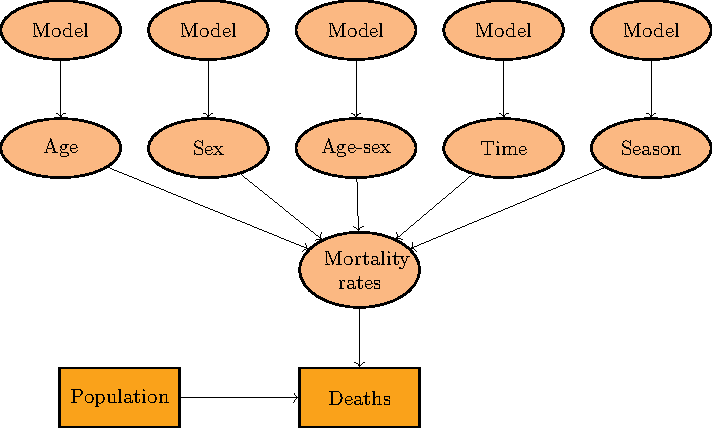
\includegraphics[width = 0.95 \linewidth]{dag.pdf}
   Bayesian hierarchical model used for estimation and forecasting
   }


   \block{\textsc{Estimates and forecasts of rates}}{
     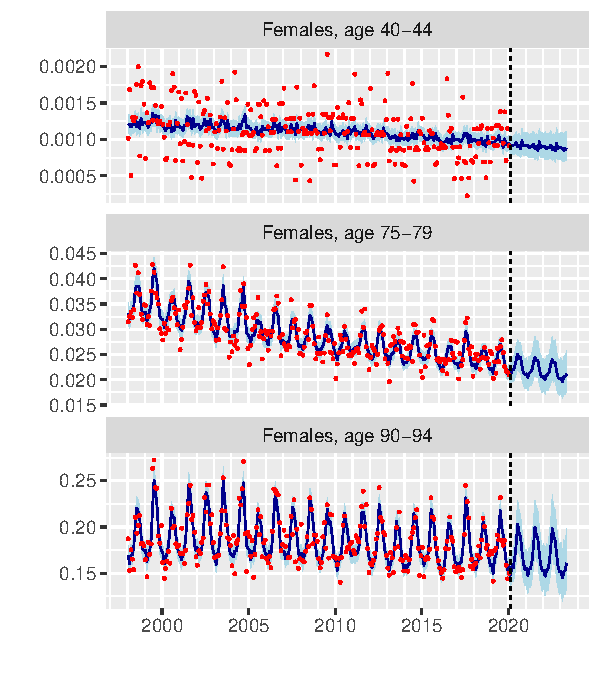
\includegraphics[width = \linewidth]{fig_forecasted_rates}
      Estimates and forecasts of mortality rates for selected groups. Blue lines and bands are point estimates and 95\% credible intervals from model. Red dots are direct estimates.
   }

   
    %%%%%%%%%%%%%%% COLONNE 2 %%%%%%%%%%%%%
    \subcolumn{.33}
    

 \block{\textsc{Calculating excess deaths}}{

    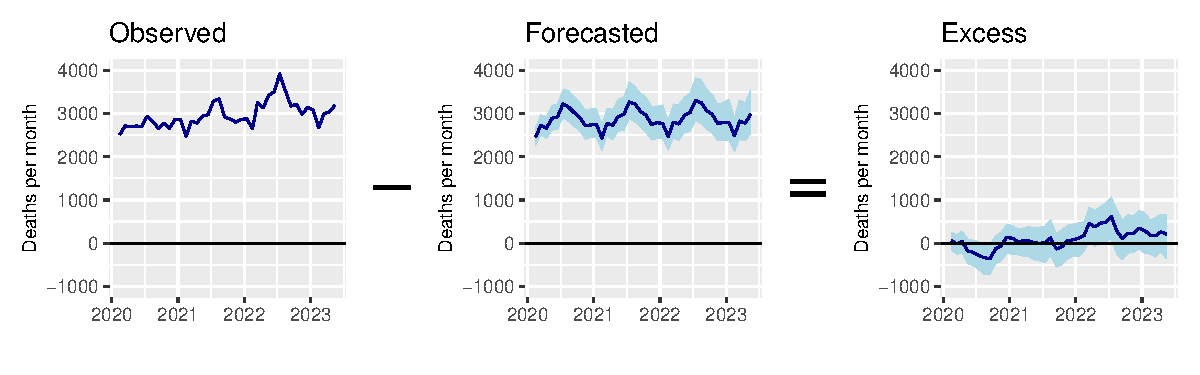
\includegraphics[width = \linewidth]{fig_calc_excess}
         Calculation of monthly excess deaths: forecasted deaths are subtracted from actual deaths
     }
            

 \block{\textsc{Excess deaths by age}}{

    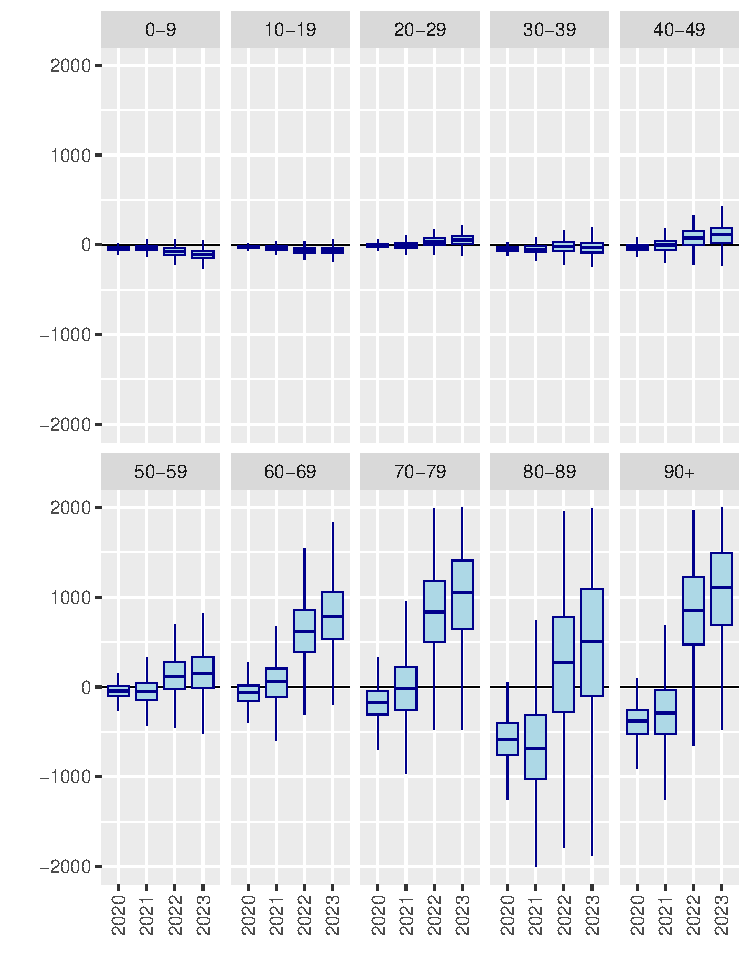
\includegraphics[width = 0.9 \linewidth]{fig_excess_age}

    Excess deaths, by age group, by year
}
            
     
        
 
 %%%%%%%%%%%%%%%%%%%%%%%% COLONNE 3 %%%%%%%%%%%%%%%%%%%%%%%%%   
    \subcolumn{.33}


   \block{\textsc{Life expectancy}}{

     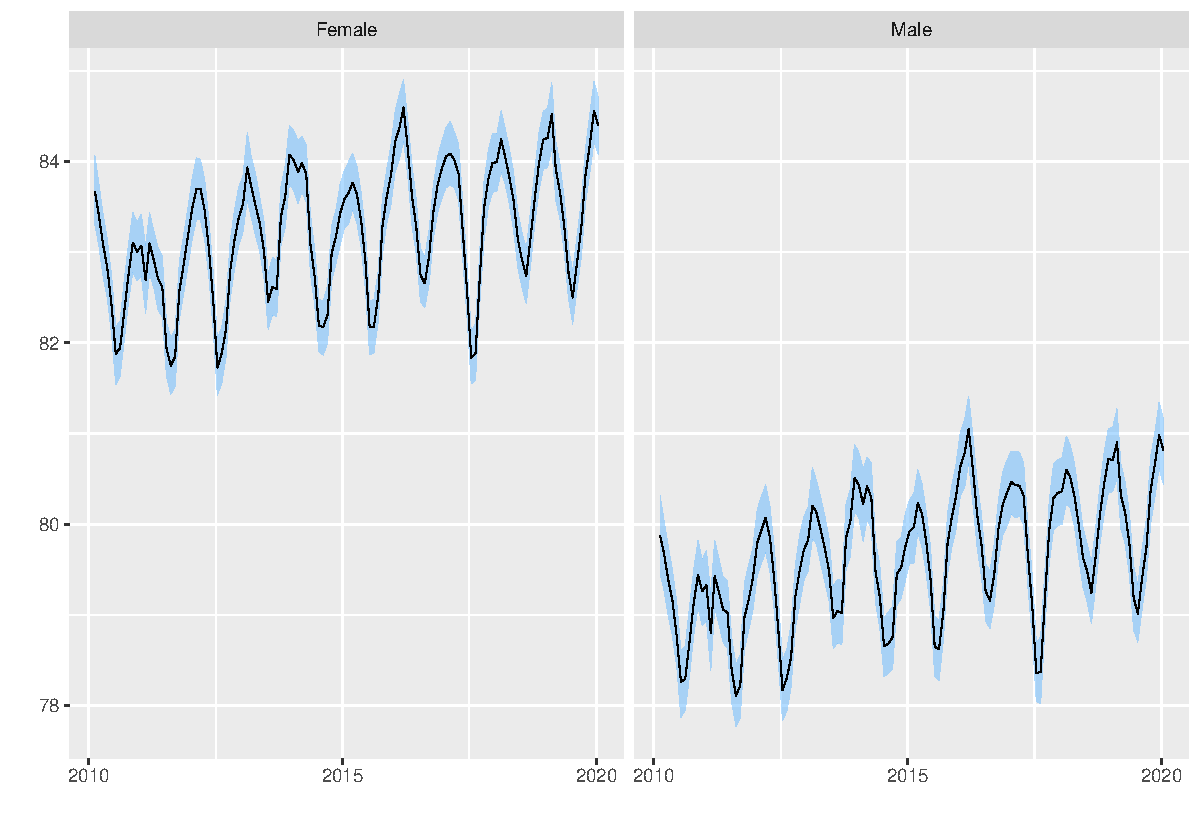
\includegraphics[width = \linewidth]{fig_lifeexp}
      Estimates of life expectancy at birth, from model fitted to data for 1998--2024
        \vspace{1cm}
   }

    
  \block{\textsc{Conclusion}}{
   \begin{itemize}
  \item Monthly excess deaths between -500 and 1000
  \item Annual excess deaths in 2022--2023 higher than 2020--2021
  \item Excess deaths concentrated among older people
  \end{itemize}
        \vspace{1cm}
 }


 \block{\textsc{Notes}}{
\begin{itemize}
\item Work in progress, and results are provisional
\item Statistical models implemented using R package \textbf{bage}
\end{itemize}
        \vspace{1cm}
  }
      
 \block{\textsc{Contact}}{
\begin{itemize}
\item  john@bayesiandemography.com
\item kim.dunstan@stats.govt.nz
\end{itemize}
 }


\end{subcolumns}
    
  \end{columns}

% ----------------- Ligne colorée à la fin du document -------------
\node [above right, text=white,outer sep=45pt,minimum
width=\paperwidth, align=center, draw, fill=titledarkcolor,
color=Orange] at (-43.6,-61) { };

\end{document}
